\subsubsection{Multilayer Perceptron}
\label{sec:mlp-multilayer-perceptron}
A multilayer perceptron consists of multiple perceptrons divided into layers and solves complex tasks \cite{Bishop1995}.
It is a universal approximator for every function \cite{Cybenko1989} regardless of the activation functions used \cite{Hornik1991}.
Because of the multiple layers and the non-linear activation functions non-linearity is introduced into the network.
Thus, it can distinguish data that is not linearly separable as most real-world data is.

There are at least three layers.
Each layer contains several perceptrons that are not connected to each other.
However, every perceptron is connected to every perceptron of its subsequent layer.
This type of connection is called a fully-connected network.
Because the data flow within the network is only in one direction and does not contain circles, the architecture is called feedforward neural network.
A visualization of this is shown in \figref{fig:multilayer-perceptron}.
Although the weights and biases are not displayed for clarity, they still exist and follow the same principle as with a single perceptron.
\begin{figure}
	\centering
	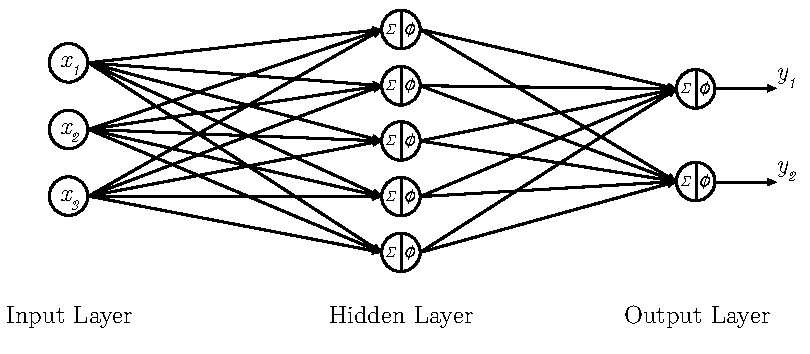
\includegraphics{images/multilayer-perceptron}
	\caption[Multilayer perceptron]{Multilayer perceptron with three layers. Each layer consists of multiple perceptrons. The input layer transfers real-world data into the network. The output layer makes the computations of the network interpretable for humans. The layers in between, the hidden layers, perform calculations and feed forward the network data. Each connection between nodes has a weight, that is not displayed for clarity. Also, every node has its own bias.}
	\label{fig:multilayer-perceptron}
\end{figure}
Like the single perceptrons every perceptron in the networks still holds its activation, a single numerical value.
A specific perceptron is referred to by its layer $l$ and position $j$ within this layer.
Hence, its activation is denoted as $a^{[l]}_{j}$.
Its weights are denoted as $w^{[l]}_{jk}$ where $k$ is the position of the preceding perceptron in layer $l-1$ and its bias as $b_j$.
All weights of layer $l$ are stored in a compact matrix $\vec{W}^{[l]}$.
In this type of network architecture perceptrons are often referred to as nodes or units.

The input layer serves as an interface for the data.
It does not perform any calculations and just passes the data to the next layer.
The number of nodes in this layer depends on the data and how it can be divided.
If the real-world data is an image, for example, the number of nodes should be equal to the number of pixels, so that every node can hold the intensity value of one pixel.

The output layer is responsible for transferring the network data to the outside so that it can be interpreted and worked with.
The number of nodes in this layer depends on the expected results.
If kinds of animals need to be detected in an image, every output perceptron would represent a single kind or category, respectively.
Assuming there are three kinds of animals possible, then there need to be three output perceptrons.
In theory, the node representing the correct kind of animal holds a one and every other a zero if the values are squashed within this range.

Every layer between the input and the output layer is a hidden layer.
They have no direct connection to the outside, neither to the input nor the output, hence, their name.
Their task is to transfer the input information to the output by performing calculations.
With at least one hidden layer every continuous function can be approximated.
So, the network models the function 
\begin{equation}
	\label{eq:multilayer-perceptron}
	f(\vec{x}) = \vec{y}
\end{equation}
where
\begin{align}
	\vec{x} = (x_0, x_1, \cdots, x_{n_x}) \\
	\vec{y} = (y_0, y_1, \cdots, y_{n_y})
\end{align}
are the input vector with $n_x$ elements and output vector with $n_y$ elements, respectively.
Every element represents the activation of a neuron in the input layer or output layer, respectively.

For the next example again an image is used.
The task is to classify a handwritten digit from the MNIST dataset \cite{Lecun98}.
\begin{figure}
	\centering
	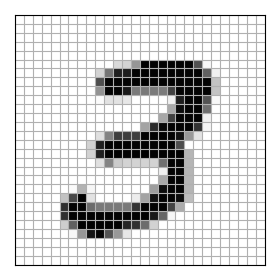
\includegraphics[]{images/mnist_digit_3a.png}
	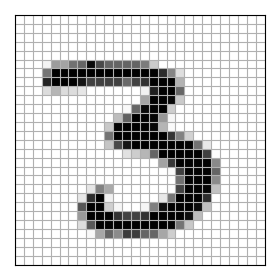
\includegraphics[]{images/mnist_digit_3b.png}
	\caption[Handwritten digits from the MNIST digit dataset]{Handwritten digits from the MNIST digit dataset. Represented as a $28 \times 28$ pixel matrix. Each cell represents a pixel.}
	\label{fig:mnist-digit}
\end{figure}
The digit can be seen in \figref{fig:mnist-digit}.
Each grid cell represents a pixel.
Now it is evident that the intensity data of every pixel is relevant for classifying the digit.
Thus, every pixel needs an associated node in the input layer of the network.
This real-world data is transferred into the network by flattening the intensity values of the image matrix to a vector.
Therefore, the vector contains $28 \cdot 28 = 784$ elements which equal the number of input nodes.
With the correct weights and biases, the network knows which nodes are active for a certain digit.
This means, that if in another image more or less the same pixels or nodes, respectively, have high intensities or activations, the same number needs to be classified.
The downside of the flattening is, that every relation of pixels like the position is lost, which means a loss in overall information.
The consequence of this is, that if a digit has no similar position and shape like the digits the networks know, the classification fails.
If, for example, a digit the network classified correctly is not centered anymore and downscaled to take up only halve its original size, completely different neurons are active.
And, thus, the network cannot find any correlation to the original image or its knowledge of how digits look and returns a wrong classification result.
Another severe downside is the huge number of parameters.
If the image gets larger, the number of input neurons naturally needs to be adapted.
Due to this, additional weights and biases are introduced to the network, because every input neuron is connected to every node of its subsequent layer.
This extends the finding of the optimal weights and biases and needs plenty of resources.
A better solution is provided by convolutional neural networks that are covered in \secref{sec:neural-networks-convolutional-neural-networks}.
